Para a problemática de uma fazenda vertical orientada por redes neurais foi definida a necessidade de mapear uma solução lógica de como o sistema de gerenciamento irá funcionar. O mapeamento (a partir da literatura existente) indicou duas possibilidades: no Fluxograma 1 a fazenda vertical (1) envia, por meio de sensores, os dados atuais de fluxo de água e fertilização para um banco de dados na nuvem (2). Estes dados podem ser acessados pelo cliente, por meio de software, onde o mesmo pode tomar a decisão como como devem operar o fluxo de água e fertilização da fazenda, recomeçando o ciclo.
\begin{figure}[h!]
    \centering
    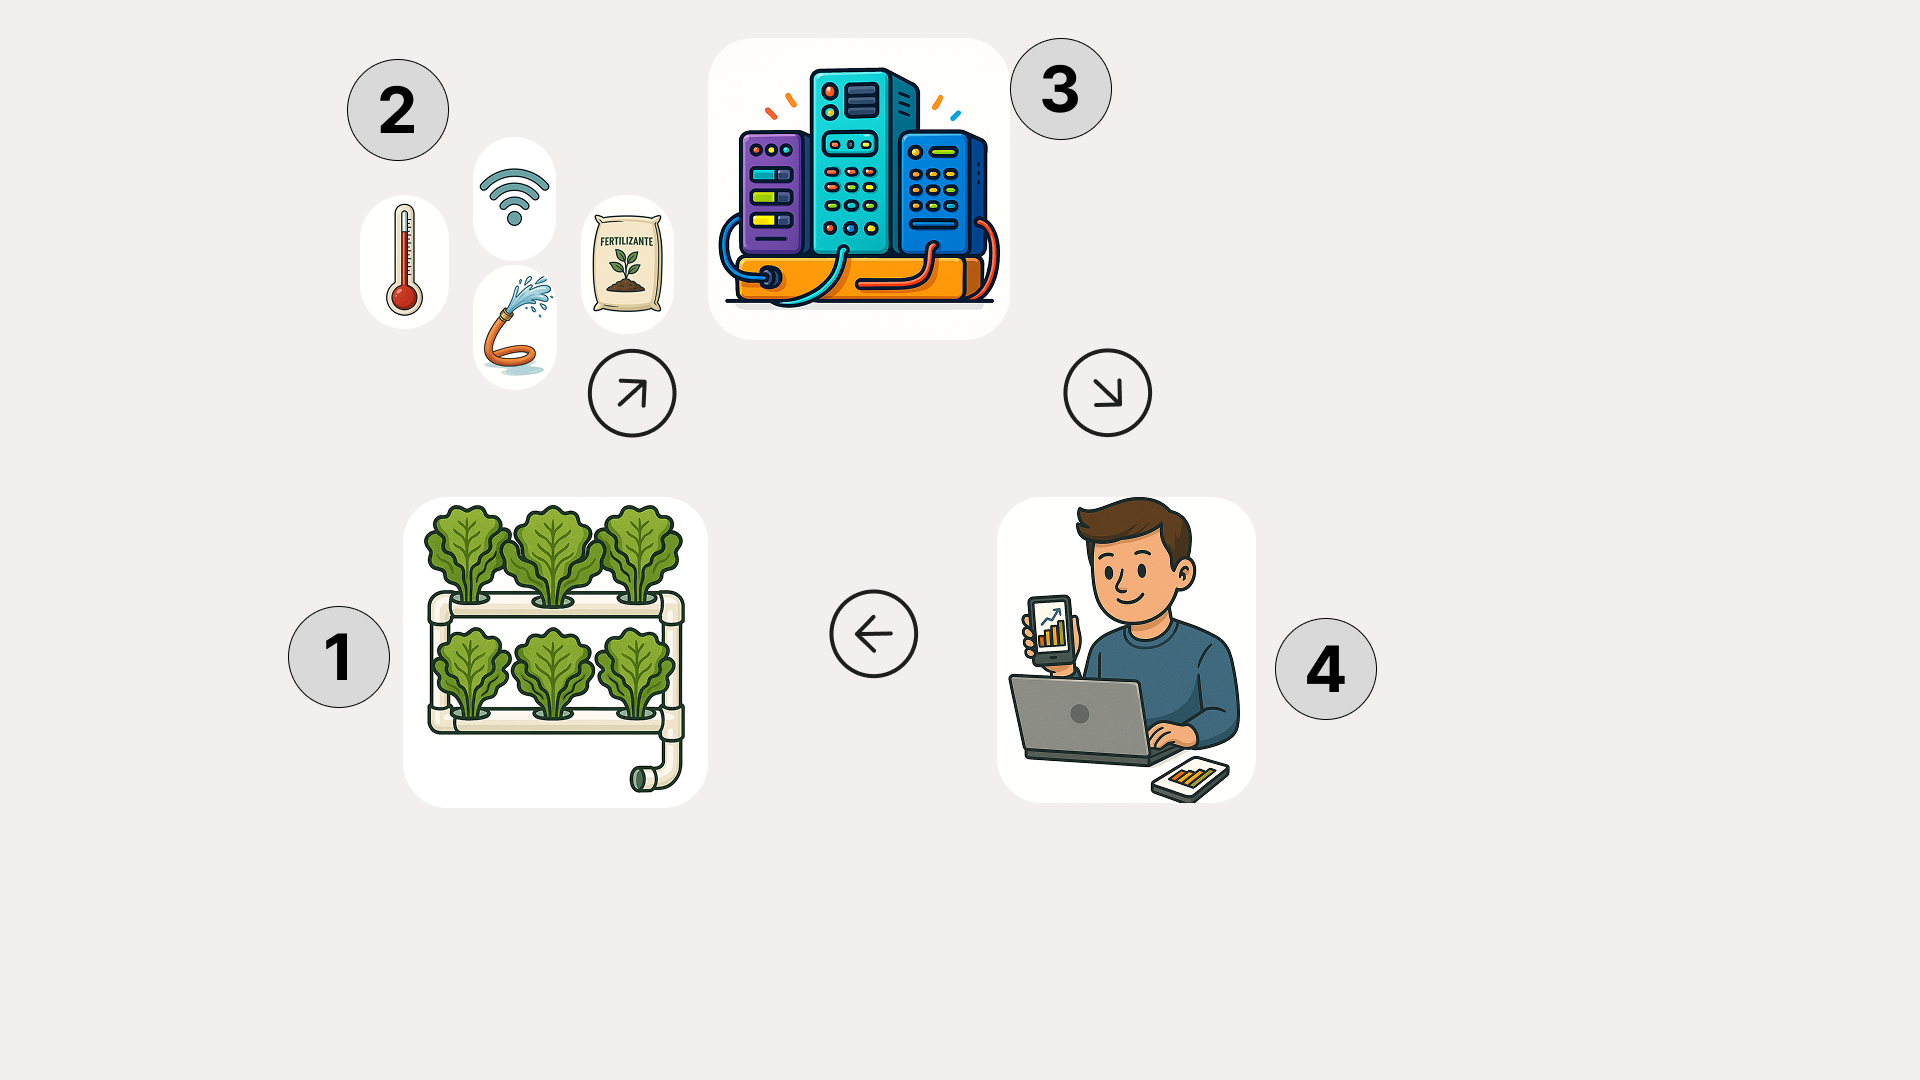
\includegraphics[scale=0.2]{Illustrations/Fluxograma1.png} % sem extensão se for .png
    \caption{Exemplo de funcionamento do sistema proposto}
    \label{fcht:fluxograma1}
    % \SourceOrNote{Autoria Própria (2024)} % só se esse comando estiver definido
\end{figure}

O Fluxograma 2 exemplifica que, inicialmente, a fazenda vertical (1) envia os dados de fertilizantes e fluxo de agua (2) para um banco de dados na nuvem (3). Porém quem faz a avaliação e tomada de decisão com base nos dados é uma Rede Neural (4), recomeçando o ciclo. Assim o cliente apenas participa do ciclo caso queira (seguindo assim o fluxograma 1).

\begin{figure}[h!]
    \centering
    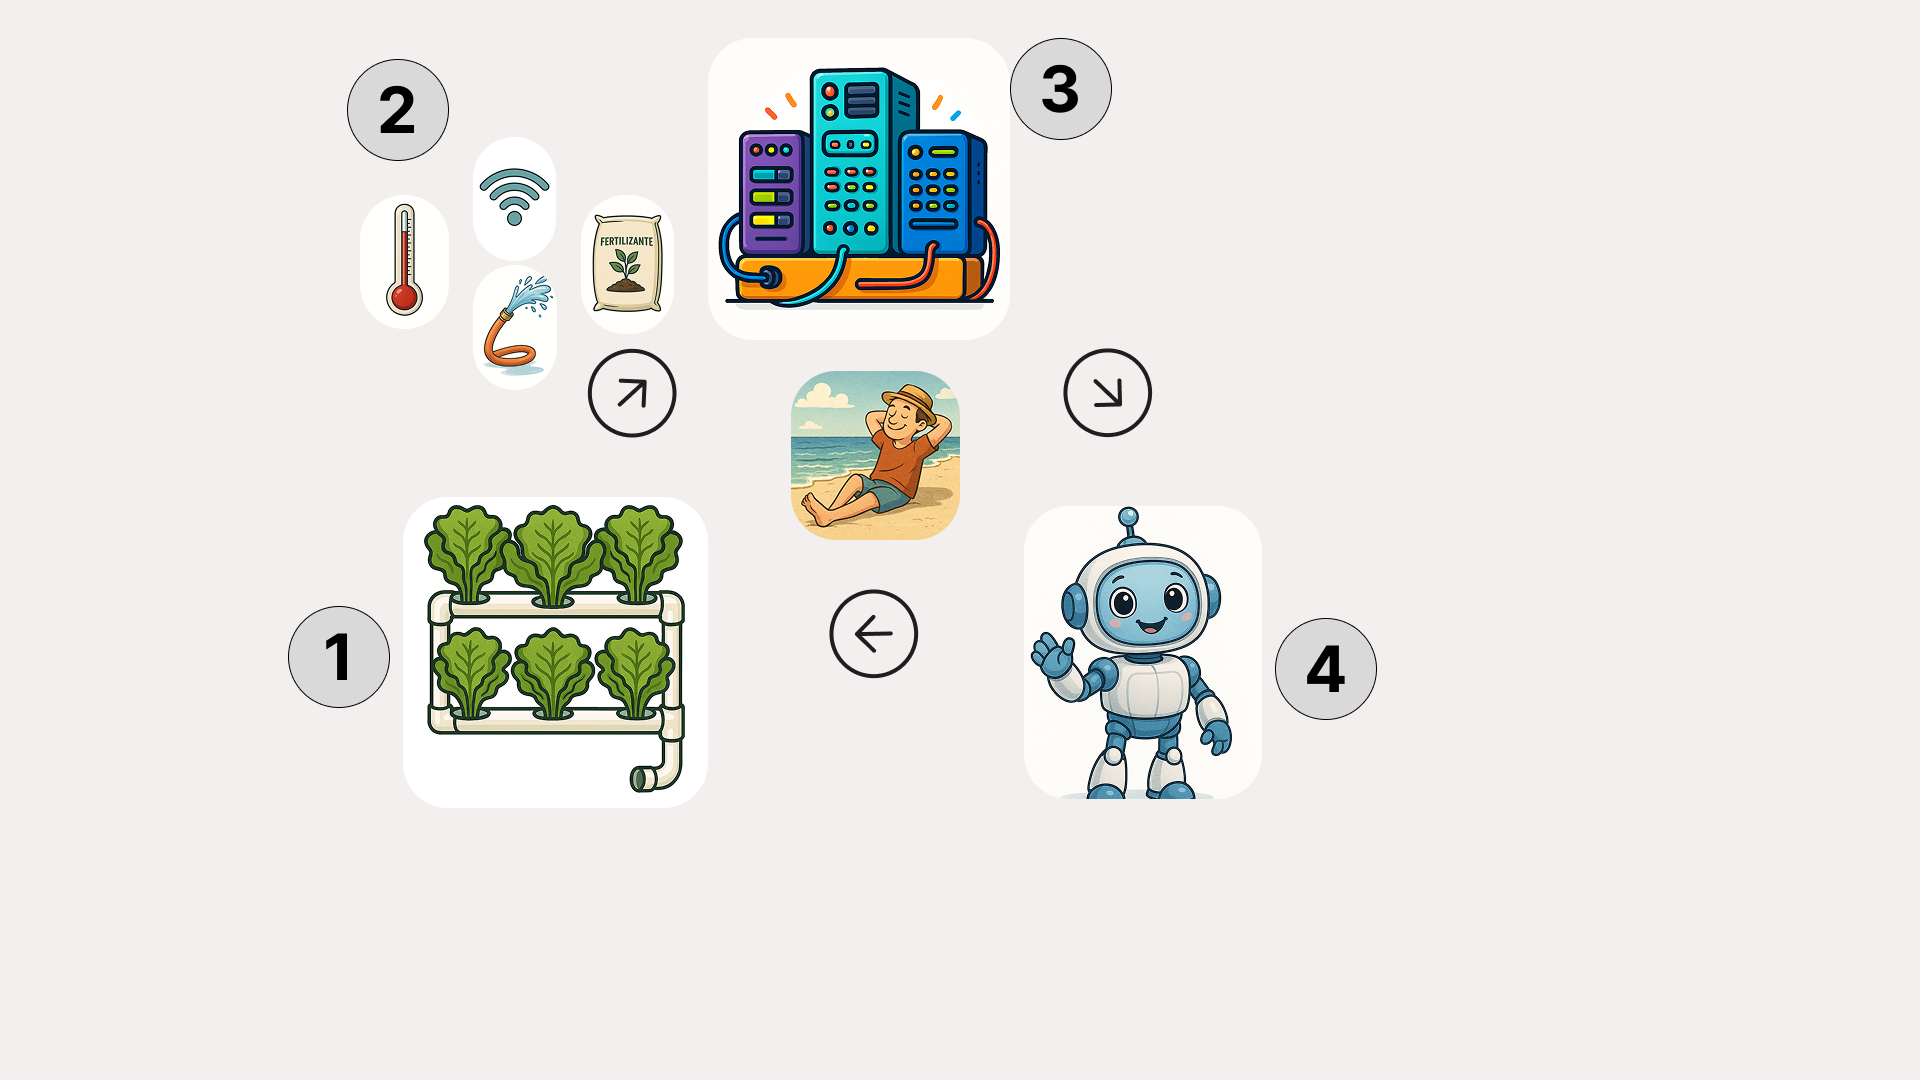
\includegraphics[scale=0.2]{Illustrations/Fluxograma2.png} % sem extensão se for .png
    \caption{Exemplo de funcionamento do sistema proposto}
    \label{fcht:fluxograma2}
    % \SourceOrNote{Autoria Própria (2024)} % só se esse comando estiver definido
\end{figure}


A seguir, são apresentadas as etapas planejadas do desenvolvimento do trabalho:

Revisão de Estudos \\
Realizado levantamento dos trabalhos mais atuais referentes a fazendas verticais, IoT, fazendas neurais e tecnologias semelhantes.

Planejamento de estrutura e definição dos componentes \\
Definição do tipo de tecnologia, armazenamento do banco de dados, layout do sistema e funcionalidades.

Construção de modelo em pequena escala \\
Elaboração de um pequeno protótipo para avaliação prática do projeto.

Implementação do sistema \\
Desenvolvimento do sistema, melhorias, testes e correções.